\documentclass[11pt,a4paper]{report}
\usepackage[utf8]{inputenc}
\usepackage[french]{babel}
\usepackage[T1]{fontenc}
\usepackage{amsmath}
\usepackage{amsfonts}
\usepackage{amssymb}
\usepackage{xcolor}
\usepackage{gensymb}

\usepackage{geometry}
\geometry{hmargin=2.5cm,vmargin=1.5cm}
\usepackage{wasysym}
\usepackage{graphicx}

\author{Mathieu Sarrat}
\title{LP16 - Microscopies optiques}

\makeatletter
\renewcommand{\thesection}{\@arabic\c@section}
\makeatother


\begin{document}
\maketitle

\section*{Pré-requis}
\begin{itemize}
	\item Optique géométrique
	\item Diffraction de Fraunhöfer
\end{itemize}

\newpage
\section*{Introduction}

Un instrument d'optique est dispositif conçu pour pallier aux limitations de l'œil. Dans cette leçon on se propose d'appliquer les notions que nous avons vues en optique géométrique pour étudier un instrument d'optique, le microscope.\\

Un microscope sert à voir de petits objets, difficiles ou impossibles à voir à l'oeil nu. Les premiers microscopes ont été conçus au $\text{XVI}^\text{e}$ siècle : Jansen, Galilée et surtout Hooke, qui dans son ouvrage "Micrographia" a décrit ses observations au sujet des puces ou des cellules végétales.\\

\begin{figure}[h!]
	\begin{center}
		\begin{tabular}{cc}
  		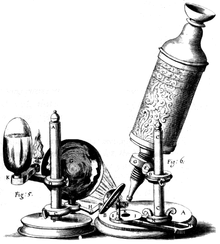
\includegraphics[scale = 0.8]{hooke_micro.png} &
   		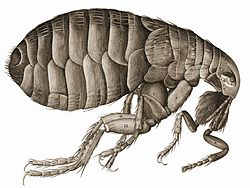
\includegraphics[scale = 0.8]{hooke_puce.png}\\
	\end{tabular}
	\end{center}
	\caption{Gauche : microscope de Hooke. Droite : gravure d'une puce.}
\end{figure}

Hooke avait conçu l'un des premiers microscopes composés, c'est à dire constitué de plus d'une lentille (trois, dans le cas du microscope de Hooke), néanmoins, compte tenu de l'importance des aberrations chromatiques et de la difficulté à les corriger, le microscope de Hooke fut globalement laissé de côté jusqu'à la moitié du $\text{XIX}^\text{e}$ siècle, au profit du microscope de Van Leeuwenhoek : une seule lentille pour un grossissement allant jusqu'à 500, pour moins d'aberrations.\\

C'est donc au milieu du $\text{XIX}^\text{e}$ siècle que les microscopes composés s'imposent, les premiers objectifs achromatiques stigmatiques (Lister) voyant le jours. Ces microscopes sont constitués :
\begin{itemize}
	\item d'un \textbf{objectif}, dont le rôle est de \textbf{collecter la lumière de l'objet et d'en 		faire une image intermédiaire},
	\item d'un \textbf{oculaire}, dont le rôle est celui d'une \textbf{loupe} observant l'image 				intermédiaire formée par l'objectif.\\
\end{itemize}

Le développement de la microscopie optique rend possible de nombreux progrès en biologie, avec notamment la découverte du noyau cellulaire par Brown en 1831, ou encore des bacilles de la lèpre par Hansen en 1874, de la tuberculose par Koch en 1882 et de la peste par Yersin en 1894.\\

De nos jours, on dispose de microscopes optiques composés très performants (plus d'aberrations) : leur résolution est limitée par le phénomène de diffraction. Le début des années 2000 a marqué un tournant avec le développement massif de techniques d'ultra-microscopies, reposant sur une nouvelle logique (on ne cherche pas à former une image mais plutôt à localiser des objets) permettant de passer outre la limite de résolution imposée par la diffraction.

\newpage
\section{Modèle de microscope composé}

Avant de nous intéresser à un système plus réaliste, nous allons d'abord présenter un modèle simplifié de microscope composé pour en comprendre le fonctionnement général. On travaillera dans les conditions de Gauss.

\subsection{Constitution}

Le modèle de microscope que nous allons caractériser est constitué de deux sous-systèmes :
\begin{itemize}
	\item l'objectif est constitué d'une lentille mince convergente 
		\textcolor{red}{indiquer la focale},
	\item l'oculaire également (\textcolor{red}{indiquer la focale}).\\
\end{itemize}

\textcolor{red}{\textbf{Construire le schéma} tout en expliquant la conjugaison :} 
\begin{itemize}
	\item l'objectif forme l'image réelle A (image intermédiaire) d'un objet réel $\text{A}_0$;
	\item dans les conditions de Gauss, l'image d'un plan est un plan, on peut donc placer le point 		B, image de $\text{B}_0$ par l'objectif, en utilisant deux rayons, passant par le foyer objet 			$F_1$ et par le foyer image $F_1'$ de l'objectif;
	\item on fait coïncider le plan focal objet de l'oculaire avec le plan de l'image intermédiaire 		AB, par conséquent l'image de AB par l'oculaire est envoyée à l'infini;
	\item on trace d'abord les rayons passant par A, puis le rayon (en pointillés) passant par B et 		le centre de la seconde lentille. On en déduit la direction avec laquelle émergent les autres 			rayons passant par B.
\end{itemize}

\begin{equation}
	\text{A}_0 \xrightarrow{\text{objectif}} \text{A} \xrightarrow{\text{oculaire}} \text{A}_i
\end{equation}

L'image finale $\text{A}_i\text{B}_i$ formée par le microscope est \textbf{à l'infini, agrandie et renversée}.

\begin{figure}[h!]
	\begin{center}
   		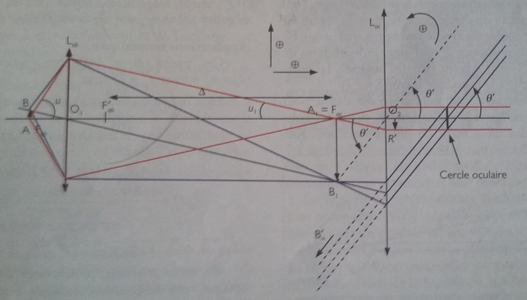
\includegraphics[scale = 0.8]{micro_principe.png}\\
	\end{center}
	\caption{Tracé des rayons dans le microscope, réglé pour un œil emmétrope observant un objet 			virtuel à l'infini.}
\end{figure}

On appelle $\Delta = \overline{F_1' F_2}$ la \textbf{longueur optique} du microscope. Cette longueur est fixée, sur un microscope réel, aussi \textbf{un microscope est équipé d'une vis micrométrique pour pourvoir faire la mise au point}, c'est à dire placer l'objet à étudier à la bonne distance de l'objectif (celle qui réalise la conjugaison que nous venons de décrire).\\

\textbf{On s'intéresse au cas où l'image finale est à l'infini, la mise au point étant faite pour un œil emmétrope (qui voit nettement à l'infini sans besoin d'accommoder).}

\subsection{Puissance intrinsèque}

On définit la puissance $P_\mu$ du microscope comme
\begin{equation}
	\boxed{P_\mu \equiv \left|\frac{\theta'}{\overline{A_0B_0}}\right|}.
\end{equation}
En multipliant et en divisant par $\overline{AB}$, on peut la relier aux caractéristiques de l'objectif et de l'oculaire :
\begin{equation}
	\boxed{P_\mu \equiv P_\text{oc} \left|\gamma_\text{obj}\right|}
\end{equation}
avec
\begin{itemize}
\item $P_\text{oc}$, la \textbf{puissance de l'oculaire}
	\begin{equation}
		P_\text{oc} \equiv \left|\frac{\theta'}{\overline{\text{AB}}}\right|
	\end{equation}
	
\item $\gamma_\text{obj}$, le \textbf{grandissement de l'objectif}
	\begin{equation}
		\gamma_\text{obj} \equiv \frac{\overline{\text{AB}}}{\overline{\text{A}_0\text{B}_0}}
	\end{equation}
\end{itemize}
L'oculaire fait office de loupe, de puissance $P_\text{oc}$. Le microscope amplifie la performance de la loupe d'un facteur $|\gamma_\text{obj}|$.\\

On parle de \textbf{puissance intrinsèque lorsque l'image finale est rejetée à l'infini}; par ailleurs, 
\begin{itemize}
	\item la trigo de base sur le triangle AB$\text{O}_2$ conduit à
	\begin{equation}
	\text{tan}\;\theta' \simeq \theta' = -\frac{\overline{AB}}{f_\text{oc}},\quad\text{d'où}\quad
	\boxed{P_\text{oc} = \frac{1}{f_\text{oc}}}
	\end{equation}

	\item théorème de Thalès avec les deux triangles $O_1IF_1'$ et $F_1'AB$ 
	\begin{equation}
		\frac{\overline{O_1I}}{\overline{AB}} = -\frac{f_\text{obj}}{\overline{F_1'A}} 
		\quad\text{or}\quad \overline{O_1I} = \overline{A_0B_0} \quad\text{et}\quad
		\overline{F_1'A} = \Delta
	\end{equation}
	d'où
	\begin{equation}
		\boxed{\gamma_\text{obj} = -\frac{\Delta}{f_\text{obj}}}
	\end{equation}
	\begin{figure}[h!]
	\begin{center}
   		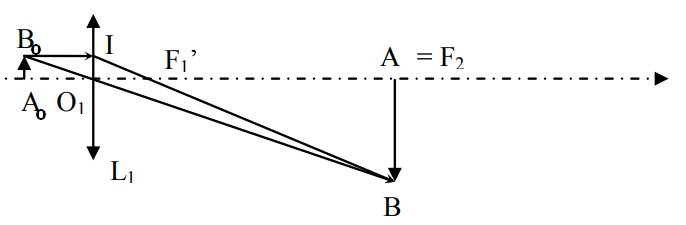
\includegraphics[scale = 0.6]{calcul_grandissement.png}\\
	\end{center}
	\caption{Pour relier le grandissement de l'objectif aux longueurs optique et focale de 					l'objectif.}
\end{figure}
\end{itemize}


On en déduit une expression de la puissance intrinsèque en fonction des caractéristiques techniques du microscope
\begin{equation}
	\boxed{P_\mu = \frac{\Delta}{f_\text{obj}f_\text{oc}}.}
\end{equation}

Dans un microscope réel, $\Delta \simeq 160$mm, fixe. Cette grandeur est bornée : la seule façon de jouer sur la puissance d'un microscope est donc de \textbf{réduire les longueurs focales}.\\

Réduire les longueurs focales implique d'augmenter l'inclinaison des rayons lumineux, et donc des \textbf{écarts importants aux conditions de Gauss}, traduits en pratique par des \textbf{aberrations}.

\subsection{Grossissement commercial}

On définit le grossissement comme
\begin{equation}
	\boxed{G \equiv \left|\frac{\theta'}{\theta}\right|},
\end{equation}
où $\theta$ désigne l'angle sous lequel l'objet $A_0B_0$ est vu à l'œil nu "au plus près", c'est à dire à la plus petite distance possible entre l'oeil et un objet pour avoir une vision nette. Cette distance, notée $d_m$ est le \textbf{punctum proximum} et vaut 25 cm pour un œil emmétrope. On a la relation suivante
\begin{equation}
	\theta \simeq \text{tan}\;\theta = \frac{\overline{A_0B_0}}{d_m} \quad\text{donc}\quad
	G = \frac{\theta'}{\overline{A_0B_0}}d_m
\end{equation}
d'où la relation entre puissance et grossissement :
\begin{equation}
	\boxed{G = P_\mu d_m}.
\end{equation}

On parle de \textbf{grossissement commercial lorsque l'image finale formée par le microscope est rejetée à l'infini}.


\subsection{Expérimentation du modèle}

\subsubsection{Profondeur de champ}

Pour qu'un œil normal (dit emmétrope) soit capable d'obtenir une image nette, l'image formée par le microscope, et donc l'objet perçu par l'œil, doit se trouver entre deux positions extrêmes :
\begin{itemize}
	\item le \textbf{punctum proximum}, situé à 25 cm,
	\item le \textbf{punctum remotum}, situé à l'infini.\\
\end{itemize}

On définit la \textbf{profondeur de champ du microscope} (ou sa latitude de mise au point) comme la distance séparant les positions de l'objet $A_0$ (notées $A_m$ et $A_\infty$ respectivement) pour que l'image formée par le microscope se trouve respectivement au punctum proximum ou au punctum remotum.\\

\textbf{Démonstration : donner la démarche et le résultat final pour gagner du temps}
\begin{itemize}
	\item \textbf{Cas où l'image formée par l'oculaire est au ponctum remotum}. 
	On a $A_0 = A_\infty$. Dans ce cas l'image intermédiaire se forme dans le plan focal objet de 			l'oculaire, d'où $A = F_2$. D'après la relation de conjugaison de Newton pour l'objectif 
	\begin{equation}
		\overline{F_1A_0}\;\overline{F_1'A} = - f_\text{obj}^2,\quad\text{qui s'écrit alors}\quad
		\overline{F_1A_\infty}\;\Delta = - f_\text{obj}^2,	
	\end{equation}
	d'où
	\begin{equation}
		\overline{F_1A_\infty} = - \frac{f_\text{obj}^2}{\Delta}.
	\end{equation}
	\item \textbf{Cas où l'image formée par le microscope est au punctum proximum}. On a $A_0 = A_m$ 		On utilise les relations de Newton pour l'objectif
	\begin{equation}
		\overline{F_1A_m}\;\overline{F_1' A} = - f_\text{obj}^2		
		\quad\text{et pour l'oculaire}\quad
		\overline{F_2A}\;\overline{F_2' A_d} = - f_\text{oc}^2, 
		\quad\text{or}\quad \overline{F_2' A_d} = -d_m	
	\end{equation}
	d'où
	\begin{equation}
		\overline{F_1A_m} = - \frac{f_\text{obj}^2}{\overline{F_1'A}} 
		= - \frac{f_\text{obj}^2}{\underbrace{\overline{F_1'A} 
		+ \overline{AF_2}}_{= \Delta} - \overline{AF_2}}
		= - \frac{f_\text{obj}^2}{\Delta + \frac{f_\text{oc}^2}{d_m}}		
	\end{equation}
\end{itemize} 
 
On en déduit la profondeur de champ
\begin{equation}
	L = \overline{A_\infty A_m} = \overline{F_1 A_m} - \overline{F_1 A_\infty} =
	\frac{f_\text{obj}^2 f_\text{oc}^2}{\Delta^2 d_m \left(1 + 
	\frac{f_\text{oc}^2}{d_m \Delta} \right)}\quad\text{en réarrangeant les termes.}
\end{equation} 

\textbf{Application numérique :} pour une longueur optique de 160 mm, un objectif de focale $f_\text{obj} = 8.0 mm$ et un oculaire de focale $f_\text{oc} = 25 mm$, on trouve une profondeur de champ d'environ 6 micromètres, d'où la vis \textbf{micrométrique} du microscope.\\

Si on veut augmenter la puissance du microscope sans toucher à l'oculaire, on doit augmenter le grandissement transversal de l'objectif, ce qui implique de réduire sa longueur focale $f_\text{obj}$ et donc sa profondeur de champ (en $f_\text{obj}^2$). Plus un microscope sera puissant, plus la mise au point sera difficile.

\subsubsection{Formation d'une image sur la rétine}

On va se placer dans la configuration où l'œil n'a pas à accommoder : l'image formée par le microscope est à l'infini, et se comporte comme un objet à l'infini pour l'œil. L'image finale va se former dans le plan focal image de la lentille que nous allons utiliser pour modéliser le cristallin. On place un écran dans ce plan.\\

\textcolor{red}{MANIP : Monter l'œil par auto-collimation pour régler l'espacement entre écran et cristallin tout en expliquant le principe, 
\begin{equation}
	A \in \mathcal{F}_o \xrightarrow{L_3} \infty \xrightarrow{M} 
	\infty \xrightarrow{L_3} A' \in \mathcal{F}_i\
\end{equation}
donc $A' \in \mathcal{F}_o$ par symétrie. Bloquer la position relative des deux pieds (barre horizontale) et placer l'œil sur le banc optique.}

\subsubsection{Mesures des caractéristiques du microscope}

\textbf{Référence :} Optique, Sylvain Houard, pages 165 à 167\\

Une fois l'œil placé, on observe une image $A_dB_d$ sur la rétine :
\begin{equation}
	\overline{A_dB_d} = -f_\text{oeil} \theta' = -f_\text{oeil} P_\mu \overline{A_0B_0}
	\quad\text{et}\quad
	\left|\gamma_d\right| = \left|\frac{\overline{A_dB_d}}{\overline{A_0B_0}}\right|
	= \frac{f_\text{oeil}\Delta}{f_1 f_2}
\end{equation}


\begin{itemize}
	\item Grandissement transversal de l'objectif
	\item Puissance de l'oculaire
	\item Puissance intrinsèque
	\item Ouverture numérique
	\item Profondeur de champ (facultatif)
	
\end{itemize}

\newpage
\section{Limite de résolution}

On appelle \textbf{résolution} la taille du plus petit détail observable de l'objet étudié. Pendant longtemps, les aberrations chromatiques (liées au caractère dispersif du verre) et géométriques (écarts à l'optique dite de Gauss) ont limité la résolution d'un microscope. Nous allons nous intéresser maintenant à un objectif et à un oculaire plus réalistes, conçus pour s'affranchir autant que possible des aberrations.

\subsection{Objectif réel}

L'objectif est la \textbf{pièce majeure du microscope}. C'est lui qui révèle les détails de l'image microscopique avec toutes ses qualités mais aussi ses imperfections. L'image fournie par les premiers objectifs composés était entachée de nombreux défauts si bien que pendant longtemps on leur préféra les microscopes simples.\\

Il existe des objectifs dits \textbf{à sec}, utilisés directement dans l'air, et des \textbf{objectifs à immersion}, qui permettent d'obtenir des grandissements plus importants mais à condition de mettre leur face avant dans un liquide (huile, glycérine) de même indice que la première lentille de l'objectif.

\subsubsection{Ouverture numérique}

La caractéristique la plus importante d'un objectif est son \textbf{ouverture numérique}, car nous verrons qu'elle conditionne son pouvoir de résolution. On la définit comme
\begin{equation}
	\boxed{\omega_0 = n_0\;\text{sin}\;u_0} 
\end{equation}
où $n_0$ est l'indice du milieu objet ($= 1$ pour un objectif à sec) et $u_0$ le demi-angle d'ouverture du faisceau incident sur l'objectif. \textcolor{red}{Schéma}.\\

Sa valeur numérique, propre à chaque objectif, est indiquée sur la monture de l'objectif (ex : 0.08, 0.22, 0.65). Un objectif à sec d'ouverture numérique de 0.65 laisse passer des rayons formant un angle d'environ $40\degree$ au plus.\\

Une telle inclinaison est bien évidemment \textbf{incompatible avec les conditions de Gauss}, or un bon objectif doit satisfaire deux conditions : être rigoureusement stigmatique et être achromatique.\\

\subsubsection{Stigmatisme rigoureux et achromatisme}

Un objectif réel est donc un système bien plus complexe qu'une simple lentille convergente comme dans le modèle précédent. Son fonctionnement repose sur une optique non paraxiale, c'est à dire qui ne respecte pas les conditions de Gauss. Un objectif réel est constitué :\\
\begin{itemize}
	\item d'une \textbf{lentille boule} : c'est un dioptre air verre sphérique, caractérisé par un 				couple de points rigoureusement stigmatiques, appelés \textbf{points de Weierstrass} et notés 		W et W'. La lentille boule est souvent coupée et le morceau retiré remplacé par une couche 				d'huile d'indice optique égal à celui du verre de la lentille.
	\item d'un ou plusieurs \textbf{ménisques d'Amici}, chargés de rabattre les rayons vers l'axe 				optique et donc de réduire leur inclinaison par rapport à cet axe.
	\item d'un ou deux \textbf{doubles achromatiques de Lister}, qui rabattent eux aussi les rayons 			vers l'axe optique, leur conférant une inclinaison compatible avec l'optique de Gauss.\\
\end{itemize}

Les doublets de Lister sont constitués d'une lentille convergente et d'une lentille divergence, dont les verres et la courbure sont choisis pour \textbf{supprimer l'aberration chromatique}.

Ce système permet d'utiliser des ouvertures numériques plus importantes que si l'objectif n'était constitué que d'une seule lentille convergente.

\subsection{Oculaire réel}

L'oculaire joue le rôle d'une loupe grossissant l'image intermédiaire. Un oculaire classique est constitué d'un double de lentilles non accolées :
\begin{itemize}
	\item un \textbf{verre d'œil}, situé du côté de l'œil
	\item un \textbf{verre de champ}, situé du côté de l'objectif.
\end{itemize}

Le fait d'utiliser un doublet permet de \textbf{corriger l'achromatisme d'une lentille simple}. Le verre de champ a, de plus, une autre utilité, celui d'\textbf{élargir le champ de vision}.

\subsubsection{Diaphragme de champ [Manip du verre de champ]}

L'oculaire ne prélève qu'une partie de l'image, il joue le rôle de \textbf{diaphragme de champ}, en bloquant une partie des rayons lumineux : ceux qui partent de la périphérie de l'objet observé.\\

Pour élargir le champ de l'instrument, on peut ajouter une \textbf{lentille auxiliaire}, appelée \textbf{verre de champ} dans le plan de l'image intermédiaire, ce qui ne \textbf{change pas la conjugaison} mais qui a pour effet de \textbf{rabattre les rayons vers l'axe optique}. On va donc élargir le champ observable \textcolor{red}{[MANIP : faire la manip en direct]}.

\subsubsection{Cercle oculaire [Tracé au tableau]}

Une question se pose : où placer l'œil pour recevoir un maximum de lumière ? Il nous faut pour cela déterminer la position de la \textbf{pupille de sortie}, également appelée \textbf{cercle oculaire}, \textbf{image du diaphragme d'ouverture} par l'oculaire \textcolor{red}{[Faire le tracé]}.\\

Toute la lumière entrant par le diaphragme d'ouverture va donc ressortir par le cercle oculaire. L'introduction d'un verre de champ a tendance à rapprocher la pupille de sortie de la lentille de l'oculaire : on pratique, on doit mettre l'œil au plus près de l'oculaire.

\subsection{Limite de résolution par diffraction}

Lorsqu'il n'y a plus d'aberrations (géométriques ou chromatiques), \textbf{c'est la diffraction qui impose une limite à la résolution}.\\

Si on se place dans l'approximation de Fraunhöfer ($R^2/(\lambda D) \ll 1$ où $D$ est la distance d'observation entre l'objet diffractant et l'image), \textbf{la figure de diffraction est une tâche d'Airy qui se forme autour de l'image géométrique}. Le calcul est nettement plus compliqué que dans le cas d'une ouverture rectangulaire car il fait intervenir les fonctions de Bessel. La première annulation de l'éclairement liée à la diffraction se trouve en 
\begin{equation}
	\boxed{r_0 \simeq 0.61 \frac{\lambda}{u_1} \simeq 0.61 \frac{\lambda_0}{n_1\;\text{sin}\;u_1}}.
\end{equation}
avec $\text{tan}\; u_1 \simeq R/D$.

\begin{figure}[h!]
	\begin{center}
   		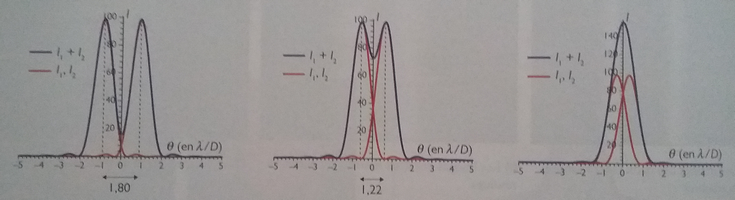
\includegraphics[scale = 0.6]{rayleigh.png}\\
	\end{center}
	\caption{Critère de Rayleigh, $\theta$ désigne l'angle sous lequel on voit un objet. Deux tâches 		d'Airy sont centrées autour des angles correspondant aux deux objets que l'on souhaite résoudre. 		Gauche : $\Delta \theta > 1.22\lambda/D$. Droite :  $\Delta \theta < 1.22\lambda/D$. Centre : cas 	limite, donnant le critère de Rayleigh. Rouge : éclairement de chaque tâche de diffraction. 			Violet, éclairement total observé.}
\end{figure}

En appliquant la relation d'Abbe entre le \textbf{plan de l'objet} et le \textbf{plan de l'image intermédiaire},
\begin{equation}
	n_0\;\overline{\text{A}_0\text{B}_0}\;\text{sin}\;u_0 
	= n\;\overline{\text{A}\text{B}}\;\text{sin}\;u,
\end{equation}
on remonte à la taille minimale $\text{A}_0\text{B}_{0,min}$ décelable pour un objet 
$\text{A}_0\text{B}_0$ :
\begin{equation}
	\overline{\text{A}_0\text{B}_{0,min}}
	=\frac{n\;\overline{\text{A}\text{B}_\text{min}}\text{sin}\;u}{n_0\;\text{sin}\;u_0}
	= 0.61 \frac{\lambda_0}{\omega_0}
\end{equation}

Plus l'ouverture numérique est grande, plus la résolution est fine, et c'est pour cela que nous avons lourdement insisté sur l'importance de l'ouverture numérique de l'objectif.

Pour abaisser au maximum cette limite de résolution, on travaille en UV ($\lambda_0 \simeq 400$nm) avec un objectif à immersion ($n_0 = 1.50$) d'ouverture numérique $\omega_0 = 1.25$, ce qui conduit à une résolution ultime d'environ 200 nm.

\newpage
\section{Battre la limite de diffraction}

Il faut donc changer d'approche si on souhaite résoudre des détails plus fins que quelques centaines de nanomètres. S'il n'est pas possible d'obtenir une image fidèle (c'est à dire des points) de deux points situés à moins de 200 nm l'un de l'autre du fait de la diffraction, il reste possible de \textbf{pointer le centre de leur tâche de diffraction}.\\

Il ne s'agît plus alors de former une image des objets émettant la lumière mais plutôt de les localiser. Ce changement d'approche est à l'origine d'une révolution en microscopie optique depuis le début du siècle, source de plusieurs prix Nobel. Nous allons présenter une technique moderne de microscopie de fluorescence à haute-résolution, la microscopie PALM/STORM.

\subsubsection{Microscopie optique de fluorescence}

La fluorescence est l'émission de lumière par une molécule \textbf{fluorochrome}, immédiatement après son excitation lumineuse, en général à une longueur d'onde plus grande (le déplacement de Stokes désigne cet écart de longueur d'onde). Le photon émis par fluorescence a une énergie plus faible que le photon absorbé). La différence d'énergie a été évacuée, par exemple sous forme de phonon lors d'une transition entre deux niveaux de vibration de la molécule.\\•

Les photons émis lors de l'émission de fluorescence n'ont pas de direction privilégiée. Il s'agit donc de choisir un objectif de grande ouverture numérique pour collecter un maximum de lumière. De plus, toutes les molécules ne sont pas fluorescentes. Il existe plusieurs techniques de marquage pour contourner ce problème. On observe les molécules d'intérêt indirectement, en repérant la fluorescence des marqueurs chromophores.

\begin{figure}[h!]
	\begin{center}
	\begin{tabular}{cc}
		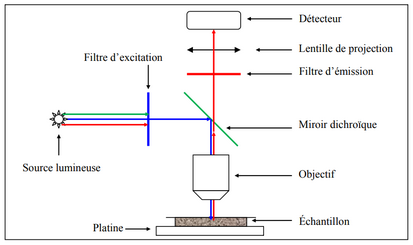
\includegraphics[scale = 0.70]{fluo_1.png} &
		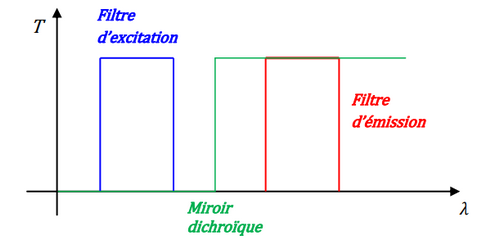
\includegraphics[scale = 0.70]{fluo_2.png}\\
	\end{tabular}
	\end{center}
	\caption{Schéma de principe d'un microscope de fluorescence : gauche, le microscope ; droite, la 		transmittance des filtres et du miroir dichroïque.}
\end{figure}

Par rapport à un microscope optique classique, on trouve des éléments supplémentaires :
\begin{itemize}
	\item un filtre d'excitation, qui sélectionne la longueur d'onde excitatrice des fluorophores de 			l'échantillon observé et bloquant les longueurs d'ondes indésirables;
	\item un filtre d'émission placé dqui laisse passer les longueurs d'ondes émises par fluorescence;
	\item un miroir dichroïque, qui réfléchit la lumière excitratrice et qui transmet la lumière émise 		par fluorescence.
\end{itemize}

L'oculaire est remplacé par une lentille de projection formant une image finale sur un détecteur, type barette CCD. Les tâches de diffraction se forment donc sur les pixels de la barette, ce qui permet de former une image. Comme la microscopie optique classique, la résolution maximale de la microscopie de fluorescence est limitée par la diffraction.\\

\textit{Remarque : fluorescence et phosphorescence désignent deux cas de luminescence. La phosphorescence perdure plus longtemps que la fluorescence.}

\subsubsection{Microscopie PALM}

La technique PALM (microscopie par localisation photoactivée), proposée en 2006 par l'équipe d'Eric Betzig (Nobel de chimie en 2014), est une technique de microscopie de fluorescence permettant de former des images d'une \textbf{résolution meilleure que la limite de la diffraction}. C'est en cela qu'on parle de \textbf{microscopie optique de "haute" résolution}.\\

Si on peut observer quelques molécules individuelles, on peut déterminer leur position avec une précision de quelques nanomètres en enregistrant tous les photons qu'elles émettent.
Pour faire une image haute résolution il faut donc marquer des molécules, faire un petit flash UV qui n'en excitera qu'un faible nombre, de récupérer la lumière émise par fluorescence et de \textbf{calculer la position du centre de chaque tâche de diffraction (centroïde)}. On répète ce processus un très grand nombre de fois en superposant à chaque fois les images obtenues.\\

Cette technique permet d'atteindre une résolution de 50 à 20 nm, soit 4 à 10 fois meilleure que la résolution prédite par le critère de Rayleigh.\\

Il existe d'autres techniques de microscopies optiques à haute-résolution : elles font l'objet de travaux de recherche fructueux en ce début de $\text{XXI}^\text{ème}$ siècle.

\section*{Conclusion}

Dans cette leçon nous avons détaillé le fonctionnement d'un microscope optique classique en nous appuyant sur l'optique géométrique. La résolution d'un tel dispositif est limitée par un effet intrinsèquement ondulatoire, la diffraction. Le critère de Rayleigh prédit une limite de résolution optique de 200 nm environ.\\ 

De nos jours, on développe des techniques de microscopie optique de haute résolution dont le principe repose sur un changement d'approche : \textbf{on ne cherche plus à former une image} au sens géométrique du terme, on repère le centre des tâches de diffraction \textbf{pour localiser des objets}.\\

Il existe enfin d'autres techniques de microscopie, exploitant d'autres types de rayonnements ou d'autres effets physiques. C'est le cas de la microscopie électronique (on exploite le comportement ondulatoire des électrons, dont la longueur d'onde est bien plus petite que celle du domaine visible) ou de la microscopie à effet tunnel.

\newpage
\section*{Annexes}
\subsection*{Microscope en réglage quelconque}
\begin{figure}[h!]
	\begin{center}
   		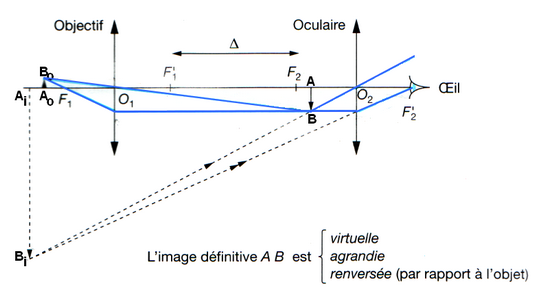
\includegraphics[scale = 0.8]{micro_general.png}\\
	\end{center}
	\caption{Tracé des rayons dans le microscope, dans le cas général.}
\end{figure}
\end{document}